

% This is sample.tex the demonstration file of
% MICCAI 2009 for Latex2e
% adapted from LLNCS.DEM from
% the LaTeX macro package from Springer-Verlag
% for Lecture Notes in Computer Science,
% version 2.2 for LaTeX2e
%
\documentclass{article}
\usepackage{spconf,amsmath,graphicx}
%
\usepackage{algorithm}
\usepackage{algorithmic}
\usepackage{amssymb,amsmath}
\usepackage{makeidx}  % allows for indexgeneration
\usepackage{url}
\usepackage{dsfont}
\usepackage{wrapfig}
\usepackage{float}
\usepackage{subfig}
\usepackage{graphicx}
\usepackage{hyperref}
\hypersetup{pdfborder={0,0,0}, colorlinks=true, urlcolor=blue}

 \graphicspath{{pics/}{figures/}}

% list here all the paths to your figure folders

\renewcommand{\topfraction}{2}
\renewcommand{\dbltopfraction}{2}
\renewcommand{\bottomfraction}{2}
\renewcommand{\textfraction}{.0}
\renewcommand{\floatpagefraction}{2}
\renewcommand{\dblfloatpagefraction}{2}

\newcommand{\argmax}{\operatornamewithlimits{argmax}}
\newcommand{\argmin}{\operatornamewithlimits{argmin}}

\begin{document}
%
%frontmatter          % for the preliminaries
%
%\pagestyle{headings}  % switches on printing of running heads
%\pagestyle{empty}  % switches on printing of running heads
%
%\mainmatter              % start of your contributions
%
\title{Automated Quantification of Morphodynamics
for High-Throughput Live Cell Time-Lapse Datasets}


%
%\author{author1\inst{1} \and author2\inst{1,2}  \and author3\inst{3}
%\name{Author(s) Name(s)\thanks{Thanks to XYZ agency for funding.}}
%\address{Author Affiliation(s)}
\name{German Gonzalez$^{1}$, Ludovico Fusco$^{2}$, Fethallah Benmansour$^{3}$, Olivier Pertz$^{2}$, Kevin Smith$^{4}$}
\address{$^{1}$ Magnetic Resonance Imaging Group, MIT \hspace{5mm} 
         $^{2}$ Institute of Biochemistry, University of Basel \\
         $^{3}$ Computer Vision Lab, EPFL \hspace{5mm} 
         $^{4}$ Light Microscopy and Screening Center, ETHZ}


\newcommand{\comment}[1]{}
\maketitle              % typeset the title of the contribution

\begin{abstract}
%% -*- mode: latex; mode: reftex; mode: flyspell; TeX-master: "top.tex"; -*-

%gg 20121023 - strengthened the findings
We present a fully automatic method  to track and quantify the morphodynamics of differentiating neurons  in fluorescence  time-lapse datasets.  Previous high-throughput studies are limited to static analysis or simple behavior. Our approach opens the door to rich dynamic analysis of complex cellular behavior in high-throughput time-lapse data. It is capable of  robustly detecting, tracking,  and segmenting all the  components of the neuron including the nucleus, soma, neurites, and filopodia. It was designed to be efficient enough to handle the massive amount of data from a high-throughput screen. Each image is processed in approximately two seconds on a notebook computer. To validate  our approach,  we analyzed over 500 neuronal differentiation videos from a small-scale RNAi screen. Our fully automated analysis of over 7,000 neurons quantifies  and  confirms with strong statistical significance static and dynamic behaviors that  had  been previously observed by biologists, but never measured. 

%Finally, we are first to
%analyze temporally the  behavior of neurons, leading to  findings not measurable
%through  state-of-the-art static  analysis. All  our findings  are statistically
%significant, with a p-value $\ll 0.05$.

%% We  present  a  fully  automatic  method to  track  and  quantify  the
%% morphodynamics of  differentiating neurons in  fluorescence time-lapse
%% datasets.     Our  approach is capable of robustly detecting,
%% tracking, and segmenting all the  components of the neuron including 
%% the nucleus, soma, neurites, and filopodia.  It is designed to be extremely efficient, capable of processing
%% each image in approximately two seconds on a conventional notebook
%% computer.  To validate our approach, we  analyzed  neuronal
%% differentiation videos in  which a set of genes  was perturbed using
%% RNA interference. Our analysis quantifes and confirms morphodynamic behaviors 
%% which had been previously observed by biologists but never measured.
%% Finally, we present new observations on the behavior of neurons made
%% possible by our analysis which could not be discovered through static analyis.


\begin{keywords}
Molecular and cellular screening; Image sequence processing; Fluorescence microscopy
\end{keywords}

%  whose
%measurements were not feasible on a large scale.  Finally, using our
%quantitative analysis we make

%our dynamic
%quantitative analysis allows us to  make new observations that are not
%visible to a human observer.


%% we  use it to  perform an siRNA  screen and
%% successfully reproduce the findings of~\cite{}, which was performed at
%% steady-state under less stressful conditions [OLVIER, HELP US SAY THIS
%%   MORE  ELOQUENTLY].   Finally, we  apply  our  approach  to make  new
%% observations   based  on  dynamic   quantitative  analysis   that  was
%% previously impossible.

%% While  previous efforts
%% have tracked the soma and nucleus,  our approach is the first to fully automatically track
%% and reconstruct the neurites as  they expand, branch and collapse, and
%% to dynamically detect fine filopodia structures.

%We present a method to analyze and extract statistics from large-scale
%video sequences  of in-vitro neurons.   Our system is able  to detect,
%track, segment  and reconstruct each individual neuron  present on the
%videos.   We show how  such system  can be  used to  find correlations
%between neuron behaviour and the proteins used to mutate them.

%high throughput automation

%confirms pre-existing findings

%yields new understandings about the dynamic morphologies

%efficient, tracks, segments, and tracks neurites


\end{abstract}

\section{Introduction and Related Work}
\label{sec:intro}
%% -*- mode: latex; mode: reftex; mode: flyspell; TeX-master: "top.tex"; -*-


The  process  of forming  functional  connections  between neurons  is
complex  and   dynamic.   Time-lapse  microscopy   has  revealed  that
differentiating  neurons undergo  a large  range of  dynamic processes
including cell body motility, filopodial dynamics, and repeated cycles
of  neurite growth  and  retraction.  Of  critical  importance is  the
process  by which  axons and  dendrites are  formed in  which a neurite
ceases retracting, extends a   long  distance, and  forms
a connection. Such  dynamic events are  governed by a  complex protein
network that  coordinates   dynamic functions 
within the cytoskeleton, membrane, etc.

Powerful tools such as 
RNA interference  (RNAi)
technology,  fluorescent  protein   labeling,  image  processing,  and
automated high-throughput  microscopy have  opened the door  for large
scale  perturbation studies to help investigate such processes. RNAi  screens have  already led  to novel
insights   into  a  number   of  cellular   processes  such   as  cell
migration~\cite{Bakal07}  and endocytosis~\cite{Collinet10}.  However,
limitations  in  image  processing  have  restricted  most
investigations to static image analysis.

Knowledge  of dynamics is  essential if we are  to understand
complex  processes such  as neuron  morphogenesis.  However, designing
algorithms to quantify dynamic  behaviors is challenging, and
automatic methods  have appeared only  very recently. State-of-the-art
high-throughput techniques have successfully quantified morphodynamics
of  HeLA cancer  cells  in an  effort  to understand 
mitosis~\cite{Held10,Neumann10,Zhu05}.   However,  the morphology  and
dynamics of  cells in previous studies are simple compared to neurons,
whose highly deformable  neurites that branch, expand,
retract, and collapse. 

%% gg 20121023 - modified greedy, added time-lapse sequence
In this paper, we propose a  fully automatic method for detecting, tracking, and
segmenting {\em  every component  of the neuron}  (nucleus, soma,  neurites, and
filopodia), and quantifying their dynamic behaviors in ways that were previously
not possible. Our  approach begins with a tracking step that detects nuclei at each  time step and
associates nuclei  belonging to the  same neuron  throughout the
time-lapse sequence.
Using tracked nuclei as  seed points, a region-growing  algorithm segments
the neuron's soma.  The somata are  used to initialize a  joint segmentation of
the entire structure  of all neurons in a  image using a probabilistic
method based on  shortest path computations.  A graph  describing the morphology
of  the neurites  is extracted  from this  segmentation.  Each  neurite  tree is
tracked by association, and filopodia  are detected by analyzing the topology of
the tracked  neurites.  Finally,  a set of  156  morphodynamic  features is
extracted, quantifying the behavior of the each neuron in the video.


As   demonstrated  in   Fig.~\ref{fig:video}, 
our  approach produces reliable  segmentations capable of capturing
complex  neuron  dynamics. To validate our approach, we analyzed a   
small-scale  siRNA screen  of 5  genes (3  siRNAs/gene). Our analysis
confirmed steady-state phenotypes obtained previously using 
MetaMorph\texttrademark~\cite{Pertz08}. We were also able to
quantify dynamic behaviors which had been previously observed, but never
measured~\cite{Pertz08}. Our  analysis also uncovered
new dynamic behaviors which are only apparant through dynamic analysis.

%While  our greedy tracking  and probabilistic  segmentation algorithms are  novel,  they are designed to be efficient and thus are relatively simple.  The  main contribution of this  paper is the  system as a whole,  which  is capable  of  high-throughput  processing of  videos, tracking individual  parts of  neurons, and quantifying  their dynamic behaviors in ways that were previously not possible.





%39ba1a
%----------------------------------------------------------------------------
\begin{figure*}[t]
       \begin{tabular}{@{\hspace{0mm}}c@{}|@{}c@{}|@{}c@{}}
        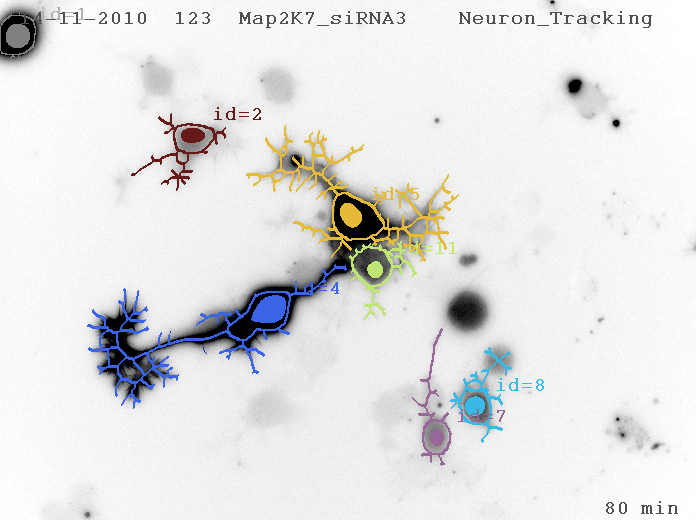
\includegraphics[width=60mm] {images/mv1_008.png} &
        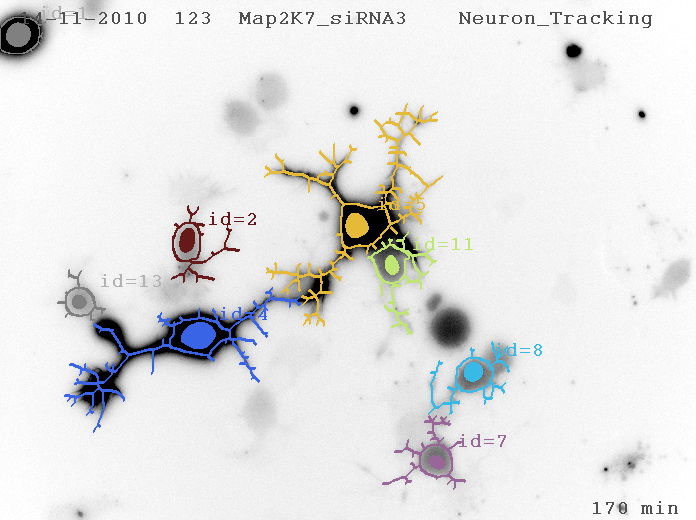
\includegraphics[width=60mm] {images/mv1_017.png}  &
        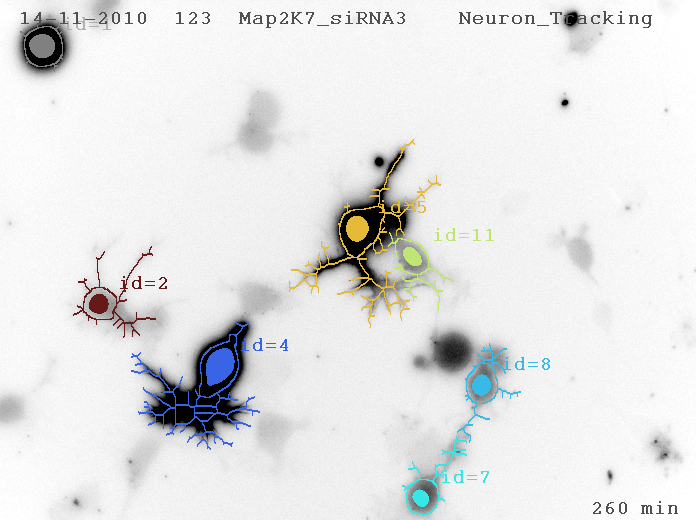
\includegraphics[width=60mm] {images/mv1_026.png} \\ [-.8ex]
        \hline \\ [-2.9ex]
       \end{tabular} 
      \begin{tabular}{@{\hspace{0mm}}c@{}c@{}|@{}c@{}c@{}|@{}c@{}c@{}}
        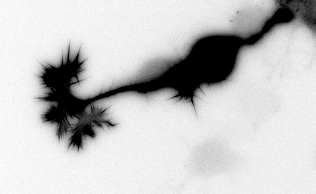
\includegraphics[width=30mm] {images/0_008.png} & 
        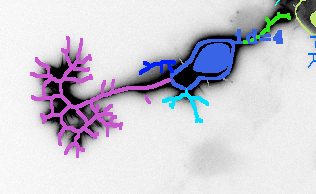
\includegraphics[width=30mm] {images/2_008_thick.png} & 
        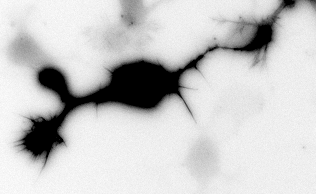
\includegraphics[width=30mm] {images/0_017.png} & 
	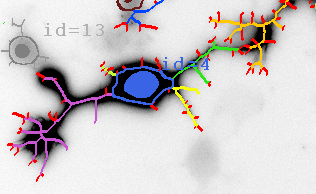
\includegraphics[width=30mm] {images/2_017_thick.png} & 
        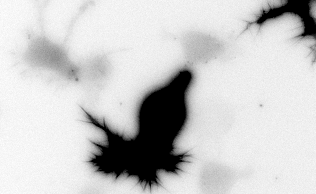
\includegraphics[width=30mm] {images/0_026.png} &
        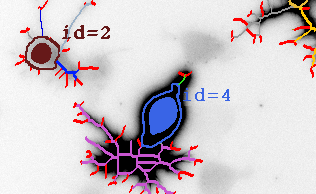
\includegraphics[width=30mm] {images/2_026_thick.png} \\ [-1ex]
	\multicolumn{2}{c}{\footnotesize $t = 80$ min} & 
	\multicolumn{2}{c}{\footnotesize $t = 170$ min} & 
	\multicolumn{2}{c}{\footnotesize $t = 260$ min} \\
      \end{tabular} 
    \vspace{-2mm}  
    \caption{\footnotesize Our approach tracks and segments the entire neuron. The top
        row contains results from an experiment with inhibited 
	MAP2K7 functions.    Tracked neurons are marked by a unique color and id.   
	Nuclei  are denoted  by  filled  ellipsoids, somata  as
        contours,  and neurites  as trees.   The bottom shows details
        from  above: the original  image on the left and  neurites
        marked with various colors on the right. Filopodia are marked in red. 
	Our  approach   performs  well  even  in  challenging
        situations where neurons appear in close proximity. Note: contrast has been 
	enhanced for visibility, faintly  stained
        cells are ignored for robustness.
	Video results can be viewed in our 
	\href{http://www.kev-smith.com/ISBI2013/}{online supplementary tables and videos}.
	}
    \label{fig:video}
\vspace{-4mm}
\end{figure*}
%----------------------------------------------------------------------------



%%----------------------------------------------------------------------------
%\begin{figure}[t]
%       \begin{tabular}{@{\hspace{0mm}}c@{}|@{}c@{}}
%        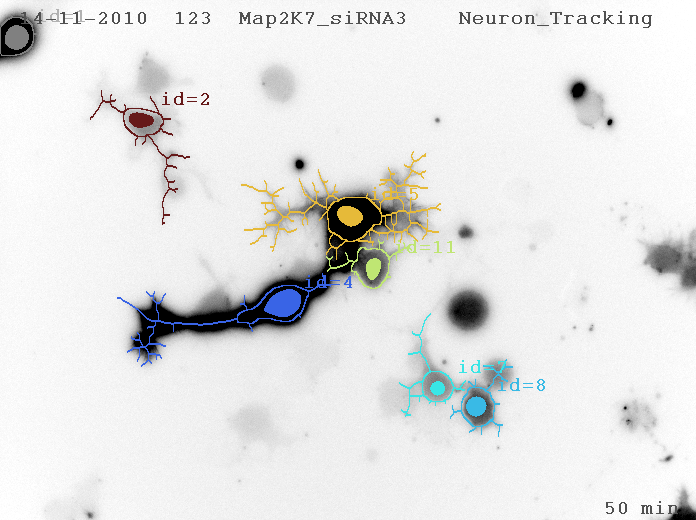
\includegraphics[width=45mm] {images/mv1_005.png}  &
%        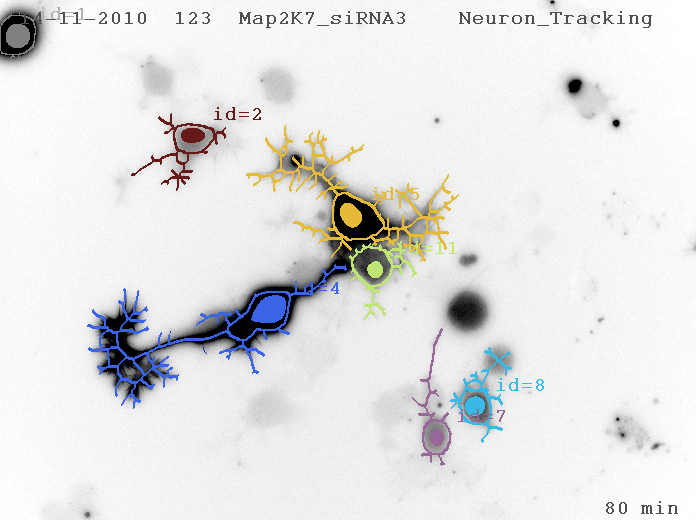
\includegraphics[width=45mm] {images/mv1_008.png} \\ [-.8ex]
%        \hline \\ [-2.6ex]
%        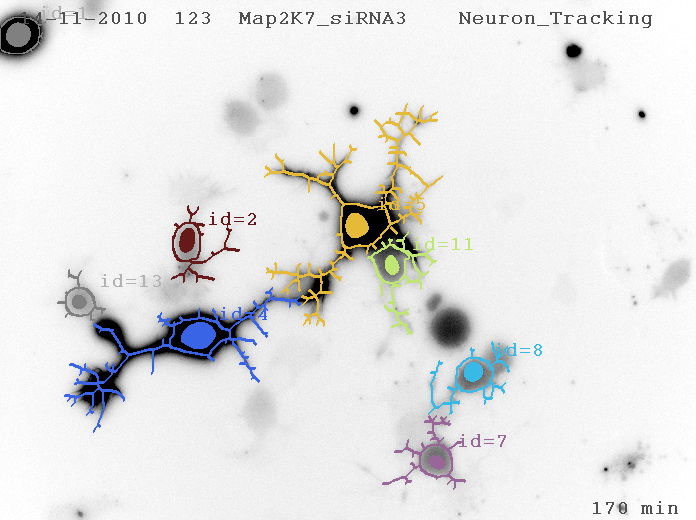
\includegraphics[width=45mm] {images/mv1_017.png}  &
%        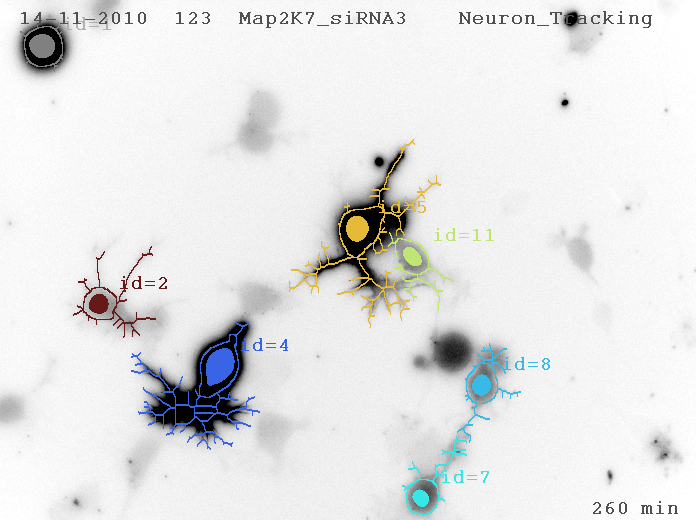
\includegraphics[width=45mm] {images/mv1_026.png} \\ [-.8ex]
%        \hline \\ [-2.9ex]
%       \end{tabular} 
%       
%      \begin{tabular}{@{\hspace{0mm}}c@{}c@{}c@{}c@{}}
%        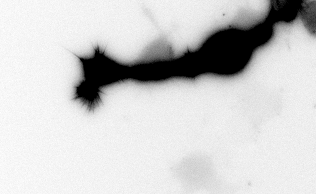
\includegraphics[width=22.5mm] {images/0_005.png} &
%        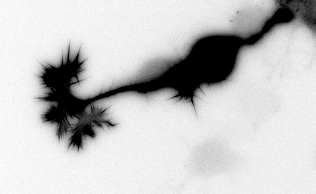
\includegraphics[width=22.5mm] {images/0_008.png} & 
%        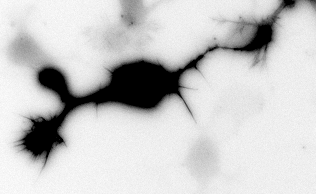
\includegraphics[width=22.5mm] {images/0_017.png} & 
%        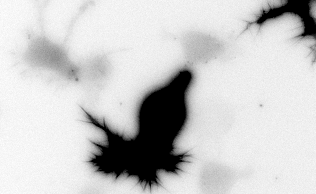
\includegraphics[width=22.5mm] {images/0_026.png} \\ [-1ex]
%        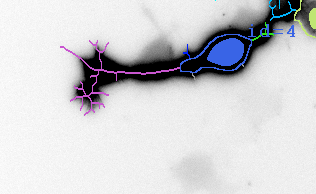
\includegraphics[width=22.5mm] {images/2_005.png} &
%        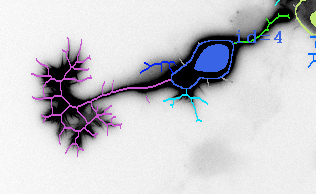
\includegraphics[width=22.5mm] {images/2_008.png} & 
%        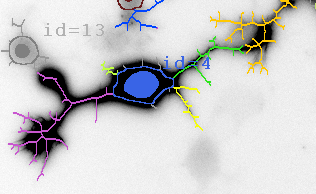
\includegraphics[width=22.5mm] {images/2_017.png} & 
%        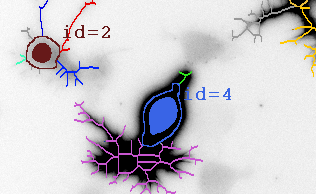
\includegraphics[width=22.5mm] {images/2_026.png} \\ [-1ex]
%        %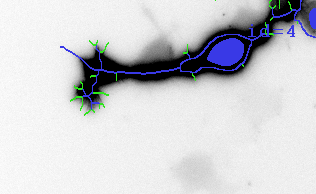
\includegraphics[width=22.5mm] {images/3_005.png} &
%        %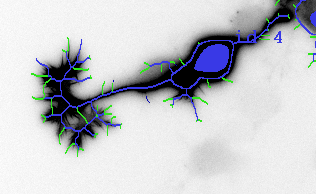
\includegraphics[width=22.5mm] {images/3_008.png} & 
%        %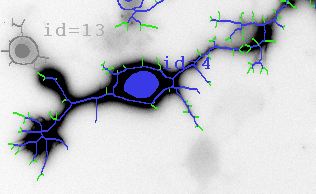
\includegraphics[width=22.5mm] {images/3_017.png} & 
%        %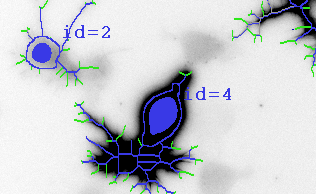
\includegraphics[width=22.5mm] {images/3_026.png} \\ [-1ex]
%        {\footnotesize $t = 50$ min} & 
%        {\footnotesize $t = 80$ min} & 
%        {\footnotesize $t = 170$ min} & 
%        {\footnotesize $t = 260$ min} \\ [-1ex]
%      \end{tabular}
%    \vspace{-2mm}  
%    \caption{ {\footnotesize {\it Neuron  Tracking Results.  } The top
%        two rows  contain frames from an experiment  where MAP2K7 gene
%        functions are inhibited.  For visibility we enhanced the image
%        contrast.  Tracked neurons are marked by a unique color and id
%        tag.   Nuclei  are denoted  by  filled  ellipsoids, somata  as
%        contours,  and neurites  as trees.   Bottom rows  show details
%        from  above: 1)  enhanced original  image 2)  tracked neurites
%        marked with a different colors. Our  approach   performs  well  even  in  challenging
%        situations where neurons appear in close proximity. Note: faintly  stained
%        cells are ignored for robustness.}}
%    \label{fig:video}
%\vspace{-6mm}
%\end{figure}
%%----------------------------------------------------------------------------




%\section{Related Work}
%\label{sec:related}
%%% -*- mode: latex; mode: reftex; mode: flyspell; TeX-master: "top.tex"; -*-


\section{High-throughput Tracking and Segmentation}
\label{sec:method}
%% -*- mode: latex; mode: reftex; mode: flyspell; TeX-master: "top.tex"; -*-

%We begin by defining the  tracking and segmentation problem along with
%some basic  notations. 

\vspace{-3mm}

The input  to our approach  is a series  of $T$ images  $\mathcal{I} =
\{I_1, \ldots, I_t,  \ldots, I_T\}$ from which we  extract $K$ nucleus
detections    $d_t^k$.     The     tracking    step    described    in
Sec.~\ref{sec:tracking} associates valid  detections across time steps
while rejecting  spurious detections. Since each  neuron contains only
one nucleus, there is a  one-to-one mapping between each valid nucleus
detection  $c_t^i$ and  a neuron  $X_t^i$. Thus,  the tracking task  is to
provide    a    set   of    neuron    detections   $\mathcal{X}^i    =
\{X_{a}^1,\ldots,X_t^i,\ldots,X_{b}^i   \}$  defining   an  individual
neuron   $i$   from   time   $t=a$   to   $t=b$.    As   depicted   in
Fig.~\ref{fig:notation}, each neuron  detection $X_t^i$ is composed of
a nucleus $c_t^i$, a soma $s_t^i$, a set of $J$ neurites $\{n_t^{i,1},
\ldots, n_t^{i,j}, \ldots,  n_t^{i,J} \}$, and a set  of $L$ filopodia
associated       with       each       neurite      $F_t^{i,j}       =
\{f_t^{i,j,1},\ldots,f_t^{i,j,l},\ldots,f_t^{i,j,L} \}$ so that $N_t^i
=  \{( n_t^{i,1},F_t^{i,1}), \ldots,(n_t^{i,j},F_t^{i,j})  \}$.  Thus,
a complete neuron $i$ is described by
$X_t^i = \{ c_t^i, s_t^i, N_t^i \}$ at time step $t$.

%Say something about how design decisions were made to keep things efficient.

%%  $N_t^i
%% =  \{(   n_t^{i,1},F_t^{i,1}),  \ldots,(n_t^{i,j},F_t^{i,j}),  \ldots,
%% (n_t^{i,J},F_t^{i,J}) \}$.

%% Each neurite $j$ associated with
%% neuron $i$ is also tracked, $\mathcal{N}^{i,j} = \{ N

%% , such
%% as $d_1$  in Fig.~\ref{fig:notation}

 %% In
%% Fig.~\ref{fig:notation} nucleus detections  appear as dark blobs.

%% In Fig.~\ref{fig:notation}  the
%% filopodia for  neurite $j=1$ are shown  in red, and  for neurite $j=2$
%% they are shown in green.

%This results in a set of 
%as described  in  Sec.~\ref{sec:detection}

%----------------------------------------------------------------------------
\begin{figure}[t]
  \begin{center}
       \begin{tabular}{c}
        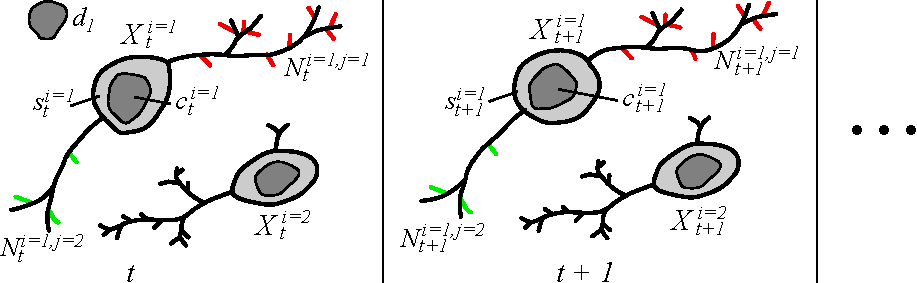
\includegraphics[width = 110mm] {images/neurondrawing.pdf}\\ [-2.4ex]
       \end{tabular} 
    \caption{  {\footnotesize  {\it Neuron  Tracking  Notation.  }   A
        neuron $i$  is defined by  a time-series of  neuron detections
        $\mathcal{X}^i     =     \{X_{a}^1,\ldots,X_t^i,\ldots,X_{b}^i
        \}$.  The  tracking returns  a  set  $\mathcal{X}^i$ for  each
        neuron $i$.  At time $t$ a neuron detection $X_t^i = \{ c_t^i,
        s_t^i, N_t^i  \}$ contains a nucleus $c_t^i$,  a soma $s_t^i$,
        and    a  set of   neurite-filopodia    tuples    $N_t^i     =    \{(
        n_t^{i,1},F_t^{i,1}),   \ldots,(n_t^{i,j},F_t^{i,j}),  \ldots,
        (n_t^{i,J},F_t^{i,J})  \}$  which  contains $J$  neurites  and
        their associated  filopodia shown in  red for $j=1$  and green
        for  $j=2$. A spurious nucleus  detection  $d_1$ is also shown.}}
    \label{fig:notation}
  \end{center}
\vspace{-9mm}
\end{figure}
%% by linking nucleus detections  and ``growing'' the
%%         neuron from the nucleus seed
%----------------------------------------------------------------------------

\subsection{Nuclei and Somata Detection and Segmentation}
\label{sec:detection}
\vspace{-2mm}
The  first  step in  our  approach  is to  extract  a  set of  nucleus
detections $\{d^1,\ldots,d^K\}$ over the  image series. We worked with
two-channel  images, one  in  which the  cytoskeleton  is marked  with
Lifeact-GFP.    In   the   other,   the   nuclei   are   marked   with
NLS-mCherry. Thus, we can reliably detect and segment nuclei by simply
thresholding  the NLS-mCherry channel  and performing  a morphological
filling operation.  In the absence  of such a channel, one could apply
a  fast machine-learning nucleus  detector such  as the  one described
in~\cite{Smith09}.


Using  the nuclei  as  seed points,  the  somata are  segmented by  an
iterative region  growing algorithm. A list of  pixels neighboring the
current  soma  segmentation is  maintained.   At  each iteration,  the
neighbor with  the smallest weighted  distance to the centroid  of the
seed  nucleus  detection  $D  =  \lambda  ||  u  -  d^k||  +  |I(u)  -
\hat{I}(d^k)|$ is added to the soma so long as $D < T$, where $u$ is a
location  in the  image,  $I(u)$  is  the pixel  intensity at  that
location, $\hat{I}(d^k)$ is the mean intensity of detection $d^k$, and
$T$ is a threshold.


\vspace{-3mm}
\subsection{Fast Greedy Tracking of Nucleus Detections}
\label{sec:tracking}
%some detections are thrown away!
\vspace{-2mm}

The tracking algorithm searches through the full set of nuclei detections
and iteratively associates the most similar  pairs of detections, returning
lists of valid detections corresponding to each neuron $\mathcal{X}^i$.
This is accomplished by constructing a graph 
$\mathcal{G}=(\mathcal{D},\mathcal{E})$  where each
node $d^k_t  \in \mathcal{D}$  corresponds to  a detection. 
For each detection $d^k_t$ in time step $t$, edges $e \in \mathcal{E}$ are formed between
$d^k_t$ and all past and future detections within a time window $W$.
A weight $w_e$ is assigned to each edge according to spatial and 
temporal distances, and a shape measure 
$w_{e} = \alpha || d^k_{t1} - d^l_{t2} ||
+ \beta |t1 - t2| + \gamma f(\nu^k_{t1}, \nu^l_{t2})$
where $e^{k,l}$ connects  $d^k_t$ and $d^l_t$, and $\nu^k$  is a shape
feature vector  containing $d^k_t$'s area,  perimeter, mean intensity,
and major  and minor axis lengths  of a fitted  ellipse. $f$ evaluates
differences between  a feature $a$ extracted from  $d^k_t$ and $d^l_t$
as  $f(a^k,a^l) =  \frac{|a^k  - a^l|}{|a^k  +  a^l|}$.  The  tracking
solution  corresponds   to  a  set  of   edges  $\mathcal{E'}  \subset
\mathcal{E}$ that minimizes the cost $\sum_{e \in \mathcal{E'}} w_e$.

%( f(a^k,a^l) + f(ma^k,ma^l) + f(mn^k,mn^l) + f(ec^k,ec^l) + f(p^k,p^l) + 
%f(\hat{I}(d^k), \hat{I}(d^l) )$

%detections found in past $t-W \ldots t-1$ and future
%$t+1 \ldots t$ time steps.

%Edges $\mathcal{E}$ fully connect detections between time steps

%%  Graph edges
%% $\mathcal{E}$ are created between  detections belonging to a different
%% time frame  in a given  time window $W$.  A cost $c_e$ is  assigned to
%% each  edge  $e \in  \mathcal{E}$  according  to  spatial and  temporal
%% distances and  shape proximity. The  tracking output corresponds  to a
%% set  of edges  $\mathcal{E'} \subset  \mathcal{E}$ that  minimizes the
%% cost $\sum_{e \in \mathcal{E'}} c_e$.

To minimize this cost function,  we adopt a greedy selection algorithm
outlined     in    Table~\ref{algo:greedy}    and     summarized    in
Fig.~\ref{fig:greedytracking}  that iteratively  selects an  edge with
minimum  cost  $\hat w_e$  and  adds  it  to the  set  $\mathcal{E}'$,
removing  future   and  past   connections  from  the   detections  $e^{k,l}$
connects. The algorithm iterates until  the minimum cost $\hat w_e$ is
greater than  a threshold $T$. The  track for neuron  $i$ is extracted
from       $\mathcal{E}'$      by      traversing       the      graph
$(\mathcal{G},\mathcal{E}')$  and appending linked  nucleus detections
to $\mathcal{X}^i$.

%~\cite{Berclaz11}

\vspace{-5mm}
%-----------------------------------------------------------------
\begin{algorithm}[h!]
\caption{Greedy tracking association algorithm}
\begin{algorithmic}[100]
%\STATE A graph $\mathcal{G}=(\mathcal{V},\mathcal{E})$ is created where each node $v \in \mathcal{V}$ is associated to a detection.
%\STATE Graph edges $(u,v) \in \mathcal{E}$ are created between detections belonging to a different time frame in a given time window $W$.
%\STATE A weight $c_e$ is assigned to each edge according to spatial and temporal distance and shape.
\STATE Start with an empty set $\mathcal{E}'$.
\REPEAT
\STATE Find edge $\hat e^{k,l}$ with minimum cost $\hat w_e$.
\STATE Add $\hat e^{k,l}$ to $\mathcal{E}'$, linking detections $d^k_{t1}$ and $d^l_{t2}$.
\STATE Remove $\hat e^{k,l}$ from $\mathcal{E}$.
\IF {$ t1 < t2 $}
\STATE Remove edges between $d^k_{t1}$ and {\em future} detections (where $t > t1$) from $\mathcal{E}$
\STATE Remove edges between $d^l_{t2}$ and {\em past} detections (where $t < t2$) from $\mathcal{E}$
\ELSE
\STATE Remove edges between $d^k_{t1}$ and {\em past} detections (where $t < t1$) from $\mathcal{E}$
\STATE Remove edges between $d^l_{t2}$ and {\em future} detections (where $t > t2$) from $\mathcal{E}$
\ENDIF
\UNTIL{$\hat w_e > T$}
\end{algorithmic}
\label{algo:greedy}
%\vspace{-6mm}
\end{algorithm}
%-----------------------------------------------------------------


%----------------------------------------------------------------------------
\begin{figure}[t]
  \centering
       \begin{tabular}{c}
        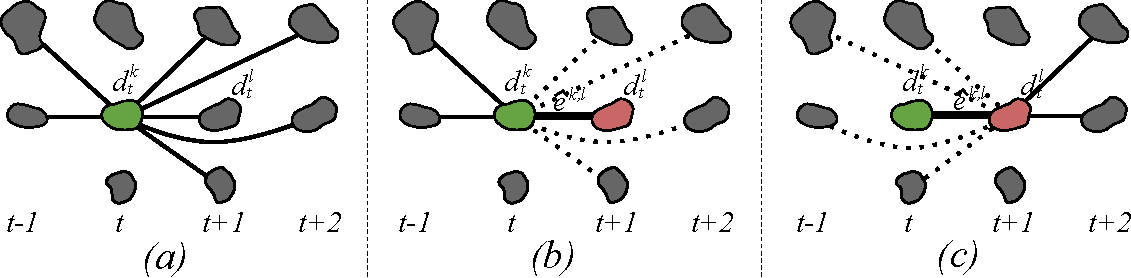
\includegraphics[width = 100mm] {images/greedytracking.pdf}\\ [-2.4ex]
       \end{tabular} 
    \caption{  {\footnotesize {\it Greedy  Tracking.}  {\em  (a)} The algorithm begins with each
        detection fully connected to all future and past detections
        within  a time  window  $W$.  Above, only  $d^k_t$'s edges  are
        shown. {\em  (b)} Each iteration,  the edge $\hat{e}^{k,l}$
        with   minimum  cost   $\hat{w}_e$  is  added  to $\mathcal{E}'$.   Edges  connecting
        $d^k_t$ to  future detections are  removed from $\mathcal{E}$.
        {\em  (c)} Edges  connecting  $d^l_t$ to  the past  are
        removed from $\mathcal{E}$.  The process is repeated until $\hat w_e > T$. }}
    \label{fig:greedytracking}
  
\vspace{-7mm}
\end{figure}
%% by linking nucleus detections  and ``growing'' the
%%         neuron from the nucleus seed
%----------------------------------------------------------------------------

\vspace{-10mm}
\subsection{Probabilistic Neuron Segmentation and Neurite Tree Extraction}
\label{sec:segmentation}
\vspace{-2mm}
Given an  image $I_t$  and the set  of somata  present in it  $S_t=\{s_t^1 \dots
s_t^m \}$,  our goal is  to associate  to each pixel  $u$ a label  $J_t(u)$ that
indicates to which soma it belongs.   The probability of $J_t(u)$ can be deduced
using Bayes' rule,
%\vspace{-1mm}
\begin{equation}
  \label{eq:bayes}
  P(J_t(u)=i|S_t,I_t) = \frac{P(S_t,I_t| J_t(u)=i)}{\sum_{\eta=1}^m P(S_t,I_t|J_t(u)=\eta)},
\end{equation}
\noindent  where we  have assumed  a uniform  distribution on  $P(J_t(u))$.  The
numerator  is modeled  as the  probability of the path $L$ that connects maximally 
the voxel $u$ to the soma $s_t^i$,
%% \begin{equation}
%%   \label{eq:shortestpath}
$  P(S_t,I_t| J_t(u)=i) = \max_{L:u\rightarrow  s_t^i}   \prod_{\{l_{r}\}
    \in L  } P(I_t(r)|l_{r}),$
%\end{equation}
where $l_{r}$ are indicator  variables for the locations forming the
path $L$. We chose this model  since an optimal maxima can be found
by minimizing its  negative likelihood using Dijkstra's shortest  path and because
it produces connected components.

To optimize this function, we map  the image  $I_t$ to  a graph  $\mathcal{G}_t^i =
(V,E)$ whose vertices  $u$ are the pixels in  $I_t$ and whose directed
edges $e_{r,v}$ connect  each pixel to its four  neighbors.  We assign
to  each edge a  weight $w_{r,v}  = -log  P(I_t(v)|v)$.  $P(I_t(v)|v)$
represents the probability that a  neurite traverses a node $v$ and is
obtained  by  applying  a  sigmoid  function  to  the  output  of  the
tubularity filter  of~\cite{Frangi98}.  The parameters  of the sigmoid
function are  estimated using  maximum likelihood. Finally,  we define
the set  of neurite pixels $U_n^t$  as those that connect  to any soma
with a higher probability than $\epsilon$.  We predict their labels as
the  ones  that  maximize   Eq.~\ref{eq:bayes}.   The  set  of  pixels
associated to neuron $X_t^i$ is the union of the neurites and the soma
associated  with $i$, $  U_i^t =  \{u \in  U_n^t |  J_t(u) =  i\} \cup
s_t^i$. To reduce  the neurite segmentation to a  tree, we skeletonize
the neuron and  define as root node the pixel  of the skeleton closest
to the centroid of the nucleus. We instantiate a Minimum Spanning Tree
from the  root and create a  neurite tree every time the  the spanning tree
exits the soma.




%\subsection{Neurite Tree Extraction}
%\label{sec:tree}

\vspace{-4mm}
\subsection{Neurite Tracking and Filopodia Detection}
\label{sec:neurite}
\vspace{-2mm}
Neurites are tracked by applying the algorithm described in Sec~\ref{sec:tracking} using
the centroids of the neurite trees instead of nucleus centroids, with the additional 
constraint that edges may only exist between neurites that emanate from the same soma.
Filopodia are detected by starting at each leaf node in a neurite and traversing the tree until a branch
point is reached. If the distance traversed is less than a threshold $T_f$, the traversed locations
are considered to be filopodia.




%% \subsection{Experiment Evaluation}

%% \subsubsection{From Image Data to Aggregates Statistics}

%% \subsubsection{Building a Distance Matrix}

%% \subsubsection{Picking the Most Discriminative Statistics}


\section{Extracting Morphodynamic Features}
\label{sec:features}
%% -*- mode: latex; mode: reftex; mode: flyspell; TeX-master: "top.tex"; -*-
\vspace{-3mm} Our  tracking and  segmentation method produces  sets of
graphs linking  detections, contours, and trees to  define each neuron
over  time.  This  data   structure  is  not  immediately  useful  for
quantifying dynamic behaviors.  To facilitate the analysis, we extract
a  set of {\em  156 meaningful  features} from  our data  structure to
quantify morphodynamics, which  are too numerous to list  here.  A few
examples  for   the  nucleus   and  soma  include:   area,  perimeter,
Lifeact-GFP  intensity,  NLS-mCherry  intensity, speed,  acceleration,
total distance  traveled, time spent  expanding/contracting, frequency
of expansion.  For neurites: number  of branches, distance from tip to
soma, filopodia  length, number of  filopodia, major axis,  minor axis
and eccentricity of an ellipse fitted to the neurite, total length, time
spent expanding/contracting, frequency of expansion (and
$\Delta$'s for all above).



\section{Results}
\label{sec:results}
%% -*- mode: latex; mode: reftex; mode: flyspell; TeX-master: "top.tex"; -*-
\vspace{-3mm}
%----------------------------------------------------------------------------
\begin{figure*}[t!]
  \centering
       \begin{tabular}{@{}c@{\hspace{2mm}}c@{\hspace{2mm}}c@{}}
         {\footnotesize (a) Maximum Distance from Neurite Tip to Soma} &
         {\footnotesize (b) $\Delta$ Neurite Elongation} &
	 {\footnotesize (c) Nucleus Speed}\\
%	 {\footnotesize (d) Maximum Number of Branches in Neurite} \\ %[-1ex]
        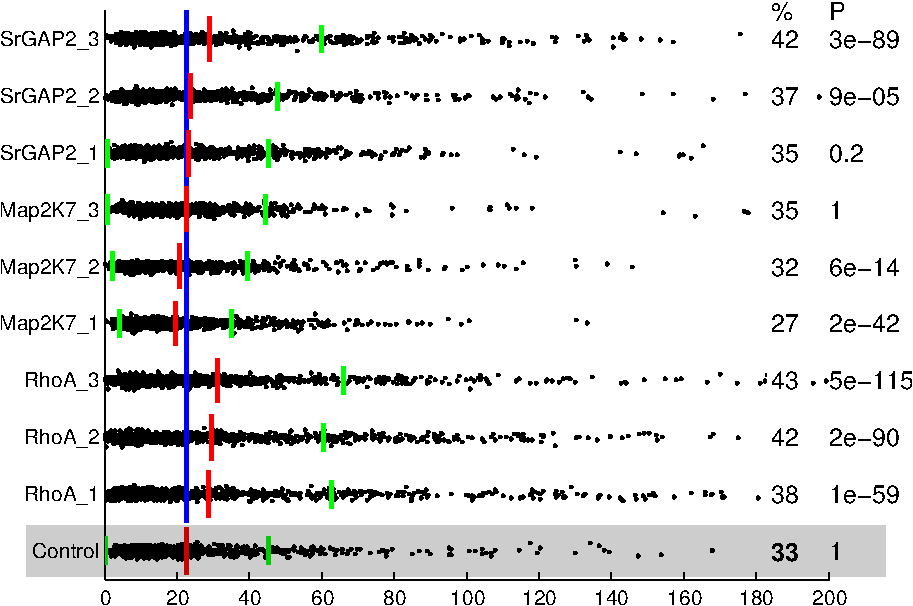
\includegraphics[height = 38mm] {images/DistToSomaExtremeNeurite.pdf} &
        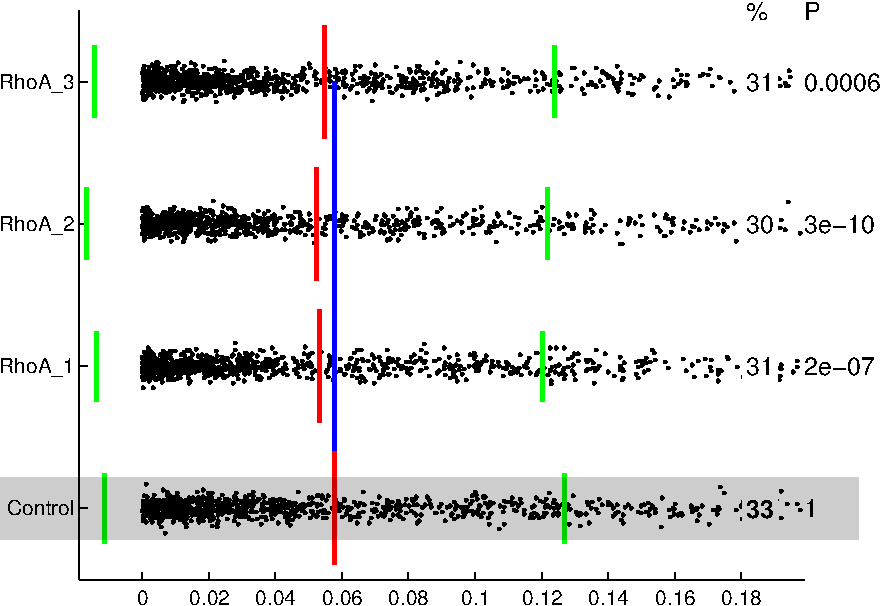
\includegraphics[height = 38mm] {images/EccentricityNeuriteDelta.pdf} &
        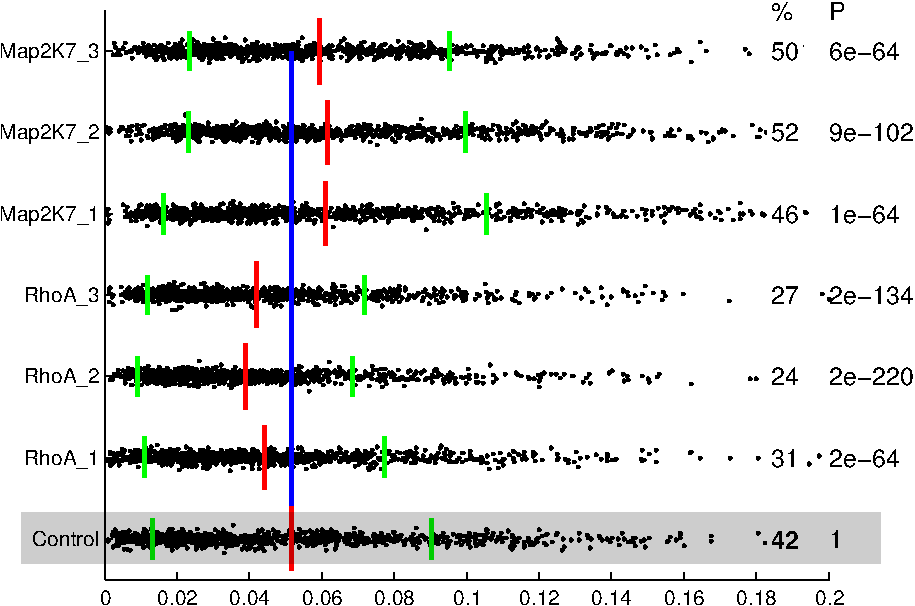
\includegraphics[height = 38mm] {images/SpeedNuclei.pdf} \\ [-1ex]
%        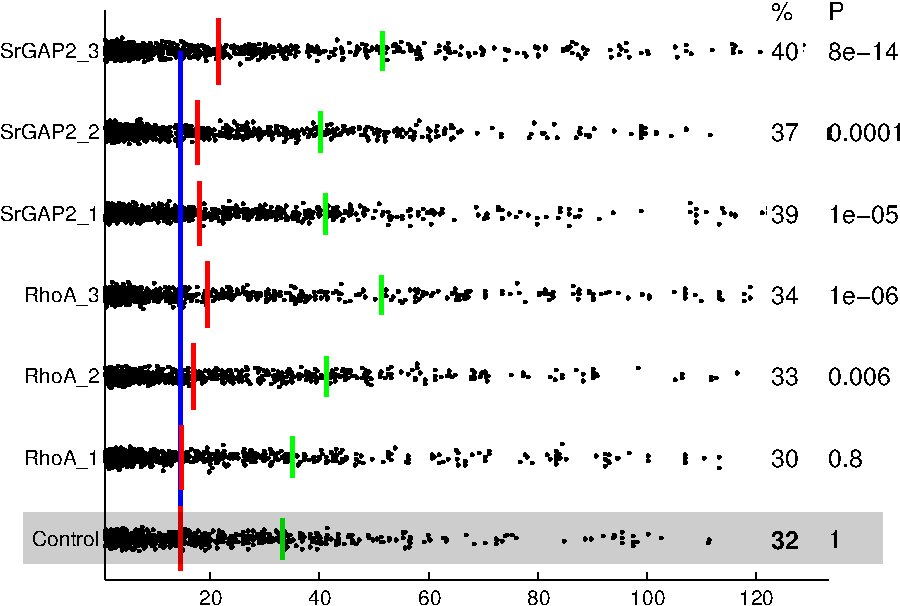
\includegraphics[height = 38mm] {images/MaxBranchCountNeurite.pdf} \\ [-1ex]
	{\footnotesize $\mu$m} & Elongation &        
%        {\footnotesize $\mu$m/min } & {\footnotesize Number of branches} \\ [-2.2ex]
	{\footnotesize $\mu$m/min } \\ [-2.2ex]
       \end{tabular} 
    \caption{ \footnotesize Morphodynamic analysis of 3/156 informative features
      out system extracts.  The control is marked in  gray.  Black dots indicate
      collected data  points.  Red bars  indicate the mean, green  bars indicate
      standard deviation.   The control  mean is shown  by a blue  line.  Values
      under the $\%$ column show the percentage of data points below the control
      mean.  The  P column  reports the statisical  signifcance measured  by the
      student-t test  $p$-value.  {\em (a)}  Our analysis confirmed  the finding
      from~\cite{Pertz08} that RhoA and  SrGAP2 loss results in longer neurites,
      and Map2K7 loss  results in shorter neurites. {\em (b)}  The low change in
      neurite elongation associated with loss of RhoA quantifies the observation
      that RhoA  loss limits the cell's  ability to retract  neurites. {\em (c)}
      Our  analysis   revealed  that  loss  of   Map2K7  and  RhoA   led  to  an
      enhancement/retardation of nucleus speed,  which was impossible to observe
      through static analysis.  }
    \label{fig:quantitative_analysis}
    %\vspace{-7mm}
\end{figure*}
%----------------------------------------------------------------------------

%% \subsection{Experimental Setup}
We applied our approach to data from a small-scale siRNA screen in which 
the functions of 5 genes were inhibited: SrGAP2, MAP2K7, RhoA, Trio, and 
Net. Three siRNAs were applied for each gene, producing a total  of 17  
experiments  including  2  controls. 30  videos  per
experiment were obtained over the  course of 3 days, with images taken
at 20$\times$ magnification 
in  10 minute intervals.  A  total of  510 videos were collected,  each containing
approximately 100 2-channel images  of $696 \times 520$ resolution.
We tracked and segmented a total of 7,298 neurons (33,213 neurites), 
extracting morphodynamic features for each. A video took under 210 seconds 
to process on a notebook computer. The entire screen was
processed in just a few hours using conventional PCs.








\subsection{Analysis}
Our goals were to 1) validate our approach by reproducing the findings 
of~\cite{Pertz08}, 2) quantify previously observed but unmeasured morphodynamics,
and 3) uncover  new dynamic behaviors.
A brief summary of our findings is provided below and in 
Fig~\ref{fig:quantitative_analysis}. Further details can be found in our 
supplementary tables and videos.
%\href{http://www.kev-smith.com/ISBI2013/}{online supplementary tables and videos}.
The findings reported below all have statistically  significant measures,  with 
a $p$-value $<< 0.05$.


Our analysis confirmed several effects previously observed through static image
analysis  in~\cite{Pertz08}.  In  particular,  RhoA  loss  of  function
resulted in fewer but longer neurites than the control. SrGap loss was
found to have longer neurites, and  Map2K7 loss was found to have
more neurites but of shorter length.  These findings  were confirmed by 
static measures from
our experiments: the mean longest  neurite length -- control $22.6 \mu
m$, RhoA-3 $32  \mu$m, SrGap2-1 $28.9 \mu$m,  and Map2K7-1 $19.5 \mu$m  
(see  Fig.~\ref{fig:quantitative_analysis}a);  and  by  a  dynamic
measure --  the mean  number of neurites  belonging a neuron  over its
lifetime: control 3.4, RhoA 3.1, and Map2K7-1 3.9.

It  had been previously observed, but  never quantified,  that  loss of
SrGap2 function  produces a  high number of  filopodia, and  that RhoA
loss  results  in neurites  that  easily  extend  but have  difficulty
retracting. Morphodynamic features from our analysis confirmed these
observations. Mean number of filopodia detected per  neurite over its lifetime was $6.69$
in the control  and $8.81$ for SrGap-3$^1$. The  mean change in elongation
as measured  by an ellipse fitted  to the neurite was  $5.7\%$ for the
control        and        $5.3\%$        for        RhoA-1        (see
Fig.~\ref{fig:quantitative_analysis}b)$^1$. While this difference may seem
small,  it is  statiscially significant due  to the  large amount  of  data collected
($p$-value is $2 \times 10^{-7}$).

Our quantitative analysis revealed new morphodynamics which
were not obvious to human  observers. We found that RhoA function loss
slowed  neuron motility and  Map2K7 increased  it.  Control cells
moved at  .30 $\mu  m / min$,  RhoA moved  at .23 $\mu  m /  min$, and
Map2K7-2     moved     at    .37     $\mu     m     /    min$     (see
Fig.~\ref{fig:quantitative_analysis}c).  We  also found that  RhoA and
SrGap  increased the  branching of  the
neurites.
%(see Fig.~\ref{fig:quantitative_analysis}d).  
Over the course
of a  neurites lifetime, the maximum  number of branches  in a control
neuron    was    14.5,   19.44    for    RhoA-3,    and   21.39    for
SrGap2-3\footnote{Only neurons containing  the  $10^{th}$  percentile  of
  longest neurites were considered.}.





%%----------------------------------------------------------------------------
%\begin{figure}[t!]
%  \centering
%       \begin{tabular}{@{\hspace{-2mm}}c@{\hspace{1mm}}c@{}}
%         {\tiny (a) Maximum Distance from Neurite Tip to Soma} &
%         {\tiny (b) $\Delta$ Eccentricity of an Ellipse Fitted to Neurite} \\
%        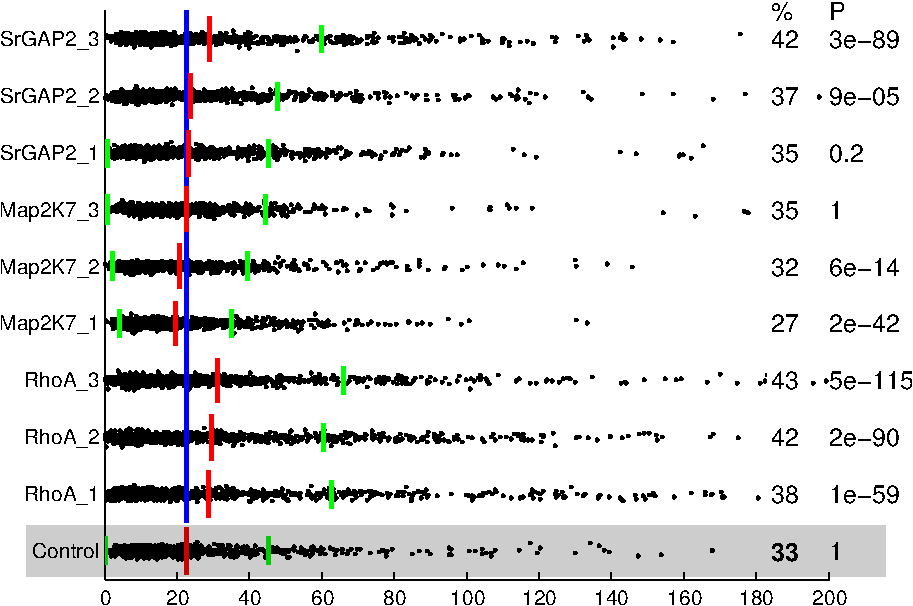
\includegraphics[height = 28mm] {images/DistToSomaExtremeNeurite.pdf} &
%        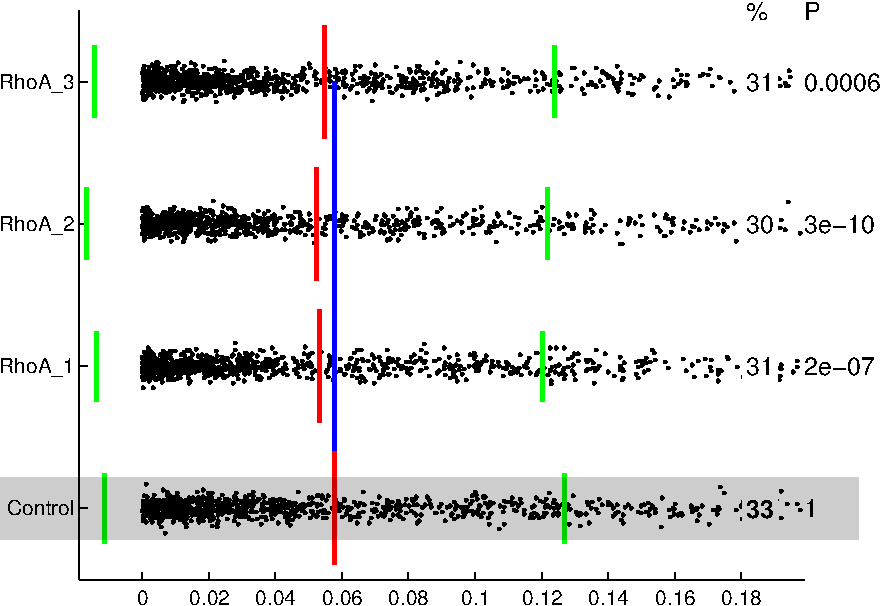
\includegraphics[height = 28mm] {images/EccentricityNeuriteDelta.pdf} \\ [-1ex]
%        {\tiny $\mu m$} & \\
%        {\tiny (c) Nucleus Speed} &
%        {\tiny (d) Maximum Number of Branches in Neurite} \\ [-1ex]
%        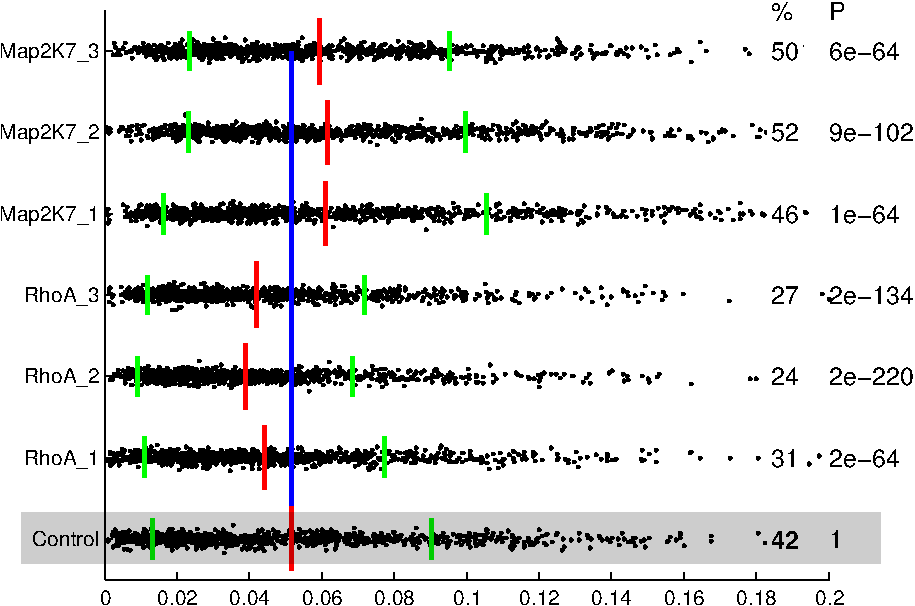
\includegraphics[height = 28mm] {images/SpeedNuclei.pdf} &
%        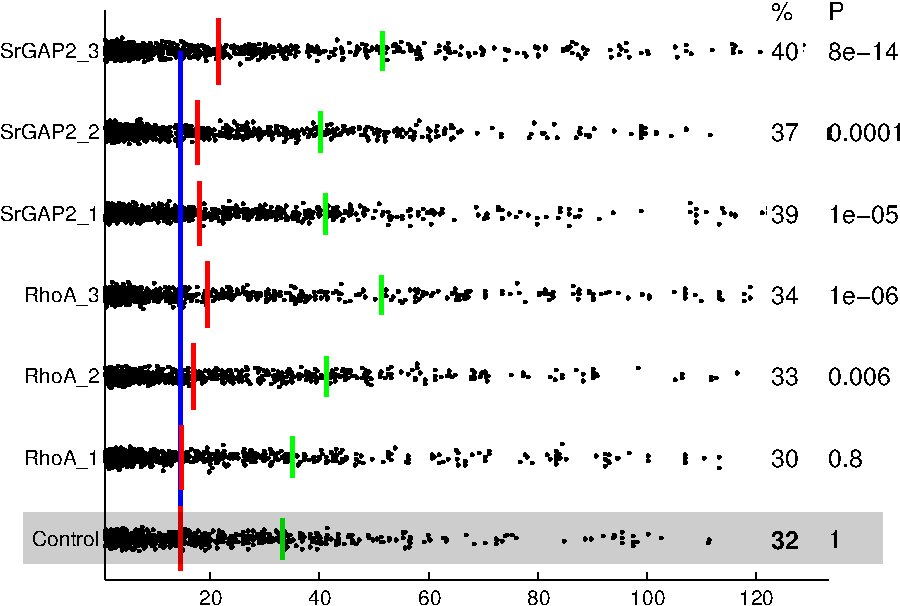
\includegraphics[height = 28mm] {images/MaxBranchCountNeurite.pdf} \\ [-1ex]
%        {\tiny $\mu m$/min } & \\ [-2.2ex]
%       \end{tabular} 
%    \caption{    {\footnotesize   {\it    Quantitative   Morphodynamic
%          Analysis.}  Four   informative  morphodynamic  features  are
%        plotted, where the control  experiment is marked in gray below
%        the  siRNA  targets.   Black  dots  represent  collected  data
%        points.  Red  bars  indicate  the mean,  green  bars  indicate
%        standard deviation.  The blue line shows the  control's mean for
%        comparison. Values under the $\%$ column are the percentage of
%        data  points  above  the  control's  mean.  Values  under  $P$
%        indicate the student-t test $p$-value. See text for details.}}
%    \label{fig:quantitative_analysis}
%    %\vspace{-7mm}
%\end{figure}
%%----------------------------------------------------------------------------






%Our analysis investigated  the effects  of  inhibiting
%various gene  functions on each  of the 156 extracted morphodynamic  features.



%Our  quantitative  analysis  investigated  the effects  of  inhibiting
%various gene  functions on each  of the 156 morphodynamic  features we
%extracted     from    our     segmentations     as    described     in
%Sec.~\ref{sec:features}.   We  summarize  our  findings below  and  in
%Fig~\ref{fig:quantitative_analysis}. We also  provide a detailed table
%and  video  results in  the  supplementary  material.  Throughout  the
%pipeline, many potential sources of noise exist, including variability
%in   neuron   behavior,   transfection   effects,  mistakes   in   our
%segmentation, and  imaging conditions.  The sheer number  of cells and
%neurites  analyzed  helps  to  average  out the  noise.  Our  findings
%reported  below are statistically  significant, all  having $p$-values
%$<< 0.05$.

%% Our approach
%% is designed to be efficient for analyzing high-throughput 
%% datasets.
%% a series of algorithm that
%% we presented

%% whole system
%% efficient

%% system is validated thorugh corroboration previous findings
%% confirmed anectocla findings
%% uncovered new dynamic phenotypes

%% biological context out of scope, future work will concentrate on that
%and addressing failure modes

%Our could be applied many other screens do more serious investiagation.


%% max branching points over  neurite lifetime
%% control  14.55
%% RhoA-3  19.44
%% SrGap2-3  21.39

%% speed
%% control   $ 9.91  \mu m / s $
%% RhoA-2    7.45
%% SrGap2-2    11.78
%% Map2K7-2   0.37
%%  0.3097    0.2328    0.3681


% eccentricity per neurite per time frame
% control 0.82
% RhoA-2 0.843  p-value  $4 \times 10^{-74}$

%% delta eccentricity
%% RhoA-1 $5.3\%$ change  $p-value$ $2 \times 10^{-7}$
%% Control $5.7\%$ change


%% over lifetime
%% RhoA_1 3.1 
%% Control 3.4
%% SrGap2_1 4.1  
%% Map2K7_1 3.9

%% 6.7 filo/neurite control



%supplementary material

%% say  how high throughput  gets rid  of noise,  and makes  our findings
%% statistically significant. talk about many sources of noise


%% p-value





%% note: make sure to say that we do not track everything - only reliably stained cells.

%% how long does it take to process?
%% It takes approximately 2.26 seconds to process each frame on a Lenovo W510 notebook computer.

%% image 97 frames 10 minute interval, 16 to 18 hours

%% In  total,  we   analyzed  $420$  video  sequences.







%\subsection{Experimental Methodology}

%\subsection{Biological Conclusions}


\section{Conclusion}
\label{sec:conclusion}
%% -*- mode: latex; mode: reftex; mode: flyspell; TeX-master: "top.tex"; -*-

We have described a fully automatic method to
track and quantify the morphodynamics of
differentiating neurons in fluorescence time-lapse
datasets.  Our approach is capable of robustly
detecting, tracking, and extracting the morphology
of the entire neuron including the nucleus, soma,
neurites, and filopodia.  Previous efforts to
analyze high-throughput screens have been limited
to static images or simple cell behavior, whereas
our approach provides researchers with a rich
dynamic analysis of complex cellular behavior in
high-throughput time-lapse data.  From the rich
set of 156 features we extract in our experiments
we are able to to 1) corroborate previous findings
by biologists, 2) quantify previously observed
neuronal behavior and 3) infer new unobserved
behaviour, all with strong statistical
significance.  

%%%%%%%%%%%%%%%%%%%%%%%%%%%%%%%%%%%%%%%%%%%%%%%%%%%%%%%%%%%%%%%%%%%%%%%%%%%%%%%%
\vspace{4mm}
\begin{centering}
\noindent {\bf Acknowledgments} \\
\vspace{2mm}
\end{centering}
%%%%%%%%%%%%%%%%%%%%%%%%%%%%%%%%%%%%%%%%%%%%%%%%%%%%%%%%%%%%%%%%%%%%%%%%%%%%%%%%
This work was supported in part by the SNF Sinergia grant
``Understanding Brain Morphogenesis'', SystemsX.ch,
the Swiss national initiative for Systems Biology,
through the SyBIT project and the Madrid-MIT M+Visi\'on consortium 
for biomedical research.



%In the future, we plan to expand
%this work to a larger scale screen and develop
%statistical techniques to infer relationships
%between genes and morphodynamic phenotypes.




%Our approach is 
%extremely efficient, and is capable of quantifying morphodynamics
%of neurons through 156 meaningful features. Using our approach, we were 
%able to reproduce previous findings from a static analysis, 
%quantify behaviors that had been previously observed but never measured,
%and uncover dynamic phenotypes. In the future, we plan to expand this
%work to a larger scale screen and develop statistical techniques to 
%infer relationships between genes and morphodynamic phenotypes.



%It is designed to be extremely efficient, capable of processing
%each image in approximately two seconds on a conventional notebook
%computer.  To validate our approach, we  analyzed  neuronal
%differentiation videos in  which a set of genes  was perturbed using
%RNA interference. Our analysis quantifes and confirms morphodynamic behaviors 
%which had been previously observed by biologists but never measured.
%Finally, we present new observations on the behavior of neurons made
%possible by our analysis which could not be discovered through static analyis.



%We have described a  set of algorithms
%which, as a  system, are capable of robustly  tracking and segmenting entire
%neurons  including  the nucleus,  soma,  neurites  and filopodia.  Our
%approach is efficient, and  can analyze high-throughput datasets using
%meaningful dynamic  features extracted from  our segmentations.
%We  validated  our  approach  by  reproducing
%previous findings,  confirming anecdotal findings,  and uncovering new
%dynamic phenotypes. It is beyond the scope of this work to comment on
%the biological significance of these findings, if there is any. We
%leave that for future work.


%\section{Conclusion}
%\label{sec:discussion}
%%% -*- mode: latex; mode: reftex; mode: flyspell; TeX-master: "top.tex"; -*-



\bibliographystyle{IEEEbib}
\footnotesize{
\bibliography{short,vision,misc,biomed}
% \bibliography{sample}
}
\end{document}








